% begin module hyperbolic-functions-def
%todo: break this into separate slides and rename appropriately 
\begin{frame}
\frametitle{Hyperbolic Functions}
Certain even and odd combinations of the exponential functions $ e^x $ and $ e^{-x} $  arise so frequently in mathematics and its applications that they deserve to be given special names.\\
In many ways they are analogous to the trigonometric functions, and they have the same relationship to the hyperbola that the trigonometric functions have to the circle.\\
For this reason they are collectively called \textbf{hyperbolic functions} and individually called \textbf{hyperbolic sine}, For this reason they are collectively called hyperbolic functions and individually called hyperbolic sine, hyperbolic cosine, and so on.
, and so on.
\end{frame}
% % % % % % % % % % % % % % % % % % % % % % % % % % % % % %
\begin{frame}
\begin{definition}[Hyperbolic Functions]
\[
\begin{array}{l@{\extracolsep{2cm}}l}
\sinh(x) = \frac{e^x-e^{-x}}{2} & \csch(x)=\frac{1}{\sinh x}\\ [3mm]

\cosh(x) = \frac{e^x+e^{-x}}{2} & \sech(x)=\frac{1}{\cosh x}\\ [3mm]

\tanh(x) = \frac{\sinh x}{\cosh x} & \coth(x)=\frac{1}{\tanh x}\\
\end{array}
\]
\end{definition}

\textbf{Note:} We will not cover inverse hyperbolic trig functions in Math 1003. 
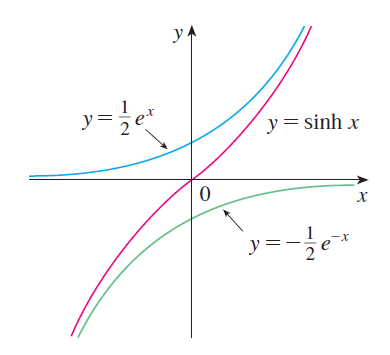
\includegraphics[width=0.35\linewidth]{../../modules/hyperbolic-functions/pictures/sinhGraph}\hfill 
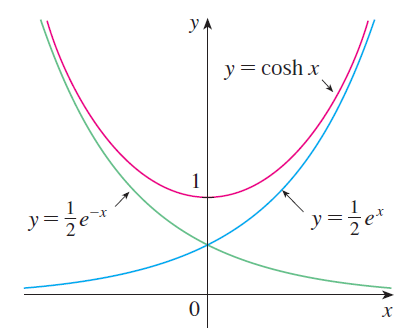
\includegraphics[width=0.35\linewidth]{../../modules/hyperbolic-functions/pictures/CoshGraph}

\end{frame}


% end module hyperbolic-functions-def
